% version 12
% Autor: Julian Salamanca
% Institución: Universidad Distrital Francisco José de Caldas
% Fecha: 09AGO2013
% Diego Alberto Parra Garzón 
\documentclass[jou]{apa6} %journal stilo APA con citacion clasica (apacite.pdf)
%\documentclass[doc]{apa6} % journal estilo latex
%\documentclass[man]{apa6}  % manuscrito APA

\usepackage[toc,page]{appendix}
\usepackage{balance}
\usepackage{multicol}
\usepackage{pdfpages}
\usepackage{afterpage}
\usepackage{float}
\usepackage{url}

\usepackage[spanish]{babel}
%\usepackage[latin1]{inputenc}% Tildes
\usepackage[utf8]{inputenc}
\usepackage{hyperref}
\urlstyle{same}

%====================================================================
%Para que no parta las palabras con guiones al final de linea
\usepackage[none]{hyphenat} 
\tolerance=6000
%====================================================================



%Stilo citaciones APA (debe ir despues de "hyperref ")
\usepackage{apacite} 

% para compilar eps con: pdflatex -shell-escape <archivo>.tex
\usepackage{epstopdf} 

\usepackage{amsmath, amsthm, amsfonts}
\usepackage{graphicx,wrapfig,lipsum}
\usepackage{anysize} 
\usepackage{fancyhdr}%
\pagestyle{fancy}
\marginsize{3cm}{3cm}{2,5cm}{2,5cm} 
%\fancypagestyle{empty}{

%  \setlength{\topmargin}{-0.5in}
%  \setlength{\headheight}{1.05in}
%  \setlength{\headsep}{0.5in}
%  \setlength{\headwidth}{\textwidth}
%  \setlength{\footskip}{2.0in}

 % \renewcommand{\headrulewidth}{0pt}

  % ========== EDITAR LOGO GRUPO =========================

%  \fancyhead[L]{
 %   \includegraphics[width=2.0cm, height=2.0cm]{LogoGI}
  %  \vspace{-1.0cm}
  %}
  % ========== FIN NO EDITAR LOGO GRUPO =================
  

  % ========== NO EDITAR LOGO UD =========================

%  \fancyhead[R]{
 %   \includegraphics[width=5.5cm, height=1.2cm]{img/logo_UD_EXT}
 % }
  % ========== FIN NO EDITAR ===========================
  

%}


\title{Un acercamiento con IoT al procesamiento y \\gestión de datos que ofrece BIG DATA }

\shorttitle{ARTICULO APLICACIÓN ANDROID}

%==================== AUTOR (ES) ========================
\author{Lic. en Física Diego Alberto Parra Garzón \\ \href{mailto:{dparra@opensai.org}}{dparra@opensai.org}}
\date{\today}
\affiliation{OPENSAI, FISINFOR}
\leftheader{Diego Parra}
%==================== FIN AUTOR (ES) ====================

%==================== RESUMEN ========================
\abstract{
\begin{center}
\textbf{Abstrac}
\end{center}



The present writing presents in an understandable and precise way the diverse dynamics that the \texttt{Opensai} team has developed in the context of \texttt{IoT}, \texttt{BigData}, science, technology and its commitment to the dissemination of them; always maintaining its free and transparent development policy by using, developing and distributing \texttt{free and open source software}; thematics that were shown to the community through the academic event \texttt{XI day of Software Uniminute}, organized by the Unit of Engineering and Basic sciences of the University Corporation Minute of God Uniminute Regional vice-rector Llanos; which started on October 20, 2017 from 7:00 to 13:00 hours, in the auditorium park of life, in the city of Villavicencio's Meta department, Colombia.


\emph{\textbf{Keywords:} } IoT, BigData, FreeSotfware, OpenSource, Science, Technology.

\begin{center}
\textbf{Resumen}
\end{center}

El presente escrito presenta de manera entendible y precisa las diversas dinámicas que viene desarrollando  el equipo de \texttt{Opensai} en el contexto de \texttt{IoT}, \texttt{Big Data}, ciencia, tecnología  y su compromiso por la divulgación de los mismos; manteniendo siempre su política de desarrollo libre y transparente al utilizar, desarrollar y distribuir \texttt{free and open source software}; temáticas que se mostraron a la comunidad a través del evento académico \texttt{XI Jornada de Software UNIMINUTO}, organizado por la Unidad de Ingeniería y Ciencias Básicas de la Corporación Universitaria Minuto de Dios UNIMINUTO Vicerrectoría Regional Llanos;  la cual tuvo inicio el día 20 de Octubre de 2017 desde las 7:00 hasta la 13:00 horas, en el auditorio del parque de la vida, en la ciudad de Villavicencio departamento del Meta, Colombia.

\emph{\textbf{Palabras Claves:} } IoT, BigData, FreeSotfware, OpenSource, ciencia, tecnología.

}


%==================== FIN RESUMEN ========================

\begin{document}

%================  NO EDITAR =================
\renewcommand{\tablename}{Tabla} %"Cuadro" por "Tabla"
\renewcommand{\refname}{Referencias} %"Cuadro" por "Tabla"
\def\st@rtbibsection{\mspart{RReferencias}}% ``References'' por ``Referencias'
\renewcommand{\rheadname}{Encabezado de página}% Running head (encabezado de pagina)
\renewcommand{\acksname}{Nota de Autor}% 
\renewcommand{\keywordname}{Palabras clave}% 
\renewcommand{\listtablename}{Índice de tablas}% 
\renewcommand{\BOthers}[1]{et al.\hbox{}}
\renewcommand{\appendixname}{Ap} %"Cuadro" por "Tabla"
\renewcommand{\appendixname}{Anexo}
\renewcommand{\appendixname}{Anexos}
\renewcommand{\appendixtocname}{Anexos}
\renewcommand{\appendixpagename}{Anexos}
\maketitle

%============== TABLA DE CONTENIDO ===============

\tableofcontents
\listoffigures
%\listoftables

%=================INTRODUCCION ============
\section{Introducción}
Las siglas \cite{gubbi2013internet} \texttt{IoT}, que proviene del idioma inglés y la cual traduce al español \texttt{internet de las cosas}, son todo el conjunto de herramientas que permiten la automatización, monitoreo, conexión y comunicación de los diversos objetos  que funcionan con electricidad, los cuales envían datos y son controlados desde \texttt{internet}.

El \cite{john2014big} BigData, es el almacenamiento, tratamiento y distintos métodos estadísticos que involucra datos por encima de un  Terabyte; esto permite a los  diferente entes gubernamentales y no  gubernamentales predecir el comportamiento de una determinada población y de esta manera obtener o brindar algún beneficio. 

En el mundo se viene desarrollando día a día diversas aplicaciones que le ofrecen a los usuarios comodidad, entretenimiento y productividad; que al combinarse con nuevas tecnologías como drones, protocolos de comunicación para diversos sensores, smart glass, teléfonos “inteligentes”, realidad virtual y aumentada, entre otros; aumentan la inmersión del ser humano en estos mundos creados por los ordenadores y visualizados por los sentidos de las personas que las utilizan; esto ha causado repercusiones en la manera que se interpreta y almacena la información, aparte ha logrado que la densidad de flujo de información que se almacena y procesa creciera de una manera exponencial, lo que desarrollo  el problema de ¿cómo analizar volúmenes de datos del tamaño de $1 x10^{21}$ bytes?; todo esto sumado al cambio de \cite{carr2011superficiales} los procesos que el cerebro humano utiliza para interpretar esta información debido a la constante inmersión de las personas en estas tecnologías; a demás loas datos \cite{perez2016peligros} que las empresas recogen para conocer a los usuarios o personas y obtener provecho de esto, recolectando, analizando y vendiendo información privada de los usuarios de una manera no informada. Pero todo no es malicia, existen múltiples personas que están comprometidas con el desarrollo de la tecnología para el beneficio de la humanidad y no el propio, dichas personas han desarrollo un número enorme de alternativas libres, no invasivas ni maliciosas, que han tenido repercusiones importantes en la vida diaria de las personas.

\section{\texttt{Internet de las cosas}}

Desde los inicios de la relación entre el internet y la automatización de diversos procesos, las personas intuían que en el futuro próximo la tecnología permitiría salvar vidas humanas, disminuir el tiempo de producción en las empresas, ayudar al campo, cuidar los recursos del planeta, entre otros; pero nadie imaginaba que las casas serian autónomas, que contarían con diversos sensores y actuadores que permitieran estar pendiente del hogar y manipularlo desde un dispositivo móvil u otro conectado a internet; tampoco que los vehículos por los cuales se movilizan diariamente para realizar sus actividades fueran controlados y vigilados desde la \texttt{nube}, nadie imaginaba que una maquina hiciera una operación mayor y critica a otro ser humano, siendo controlada por una persona al otro lado del mundo con un simulador virtual; el uso de aparatos voladores no tripulados equipados con una gama amplia de sensores y comunicación inalámbrica para ayudar a que los productos agrícolas mejoraran su calidad y vida útil.

Se utilizaron diversos contenidos audiovisuales como ejemplos para entender el alcance que ha tenido la tecnología del internet de las cosas en la vida diaria de las personas, los cuales se describen a continuación.
\begin{enumerate}
\item[*] Ciudades inteligentes unidas al internet de las cosas \footnote{Enlace en linea: \url{https://www.youtube.com/watch?v=80jVb5ae5X4}}.
\item[*] What Happens When Farming Goes High-Tech National Geographic \footnote{Enlace en linea \url {https://www.youtube.com/watch?v=tbkTi3zNN9s}}.
\item[*] Portal industrial IoT Edge para fábricas inteligentes \footnote{Enlacce en linea: \url{https://www.youtube.com/watch?v=83hamI9MvXg}}.
\item[*] Internet of Things (IoT) - SMART AGRICULTURE \footnote{Enlace en linea: \url{https://www.youtube.com/watch?v=j4HBlOf5ZDA}}.
\item[*] SAP IoT around the World \footnote{Enlace en linea: \url{https://www.youtube.com/watch?v=1ORKnjsXV48}}.
\end{enumerate}

\section{Datos masivos}
La adquisición de datos por parte de cámaras de vídeo en centros comerciales, calles, hoteles; el uso de sensores para capturar masivamente datos y otros tipos de medios de adquisición de información, tienen volúmenes enormes; toda esta información no puede ser procesada por los computadores actuales al servicio de la mayoría de la población, es por eso que surge el almacenamiento y procesamiento de datos desde la \texttt{nube}, para garantizar el progreso y avance de la población se disponen de estas nuevas tecnologías que están \cite{malvicino2014big} cambiando el modo en que se realizan los negocios desde la perspectiva del análisis estadístico y probabilístico que expertos han colocado al servicio del procesamiento de datos masivos. Se utiliza material audio-visual para visualizar el impacto del \texttt{Big Data}, los cuales se describen a continuación:

\begin{enumerate}
\item[*] Big Data Animation Video \footnote{Enlace en linea: \url{https://www.youtube.com/watch?v=rHbql-ucXqk}}.
\item[*] Big Data What it Means to You? \footnote{Enlace en linea \url{https://www.youtube.com/watch?v=-Gj93L2Qa6c}}.
\end{enumerate}

\section{Experiencia Opensai}

En este momento \texttt{Opensai} esta involucrado en diversas actividades que involucran software y hardware libre, en ellas se ve reflejado la visión y filosofía que caracteriza el compromiso de cada uno de sus integrantes y su misión de divulgar estas actividades a la comunidad en general; se describe a continuación estas dinámicas:

\begin{enumerate}
\item[*] \textbf{Prototipo de realidad aumentada basada en tecnologías emergentes para smart glass y móviles; orientado al apoyo de procesos de gestión logística en centros de distribución (Bodegas a gran escala y Zonas francas):} Este proyecto esta desarrollado para brindar un acompañamiento a los semilleros de investigación que se vienen implementando con base a estas nuevas tecnologías emergentes en el \texttt{SENA}; \texttt{Opensai} cumple la labor de no solo brindar acompañamiento, sino que también ofrece el servicio de instrucción en \texttt{IoT, BigData,} desarrollo de software múltiplataforma para implementar el control del prototipo desde sistemas de comunicación inalámbricos conectados a \texttt{Internet}, implementación de hardware libre y auto sustentable  en cuanto a su energía eléctrica se refiere pues se desarrolla con energía \texttt{foto-eléctrica} a través de paneles solares y sistemas de almacenaje de energía eléctrica con polímero de litio; \texttt{Opensai} tiene el trabajo de implementar esta aplicación en la empresa \texttt{evocom}, que tiene una bodega de almacenaje y rotación de productos tecnológicos en una de las zonas francas de Bogotá, después del puente de madera de la calle 80; cabe resaltar que todo el desarrollo esta basado para las \texttt{smarth glass} de \texttt{EPSON} o cualquier otro dispositivo; dejando como precedente haber comentado y mostrado parte de la aplicación y software de esta solución libre para logística de zonas de almacenaje para empresas y resaltando la labor y compromiso que el   \texttt{SENA} tiene con la investigación y la educación de la población Colombiana.

\item[*] \textbf{Recorrido histórico y cultural de la biblioteca Ramón Eduardo D' Luiz Nieto o biblioteca central de la Universidad Distrital Francisco José de Caldas, implementado en realidad aumentada con software libre en las gafas smarth glass BT-200 MOVERIO de EPSON. Demo: } \texttt{Opensai} en sus buenas relaciones con la \texttt{Universidad Distrital Francisco José} y específicamente en la biblioteca central que esta posee, ubicada en la carrera 30 con Avenida Jimenez  en el antiguo matadero distrital; ha desarrollado un prototipo para el recorrido con realidad aumentada para las instalaciones de la biblioteca, este recorrido cuenta con el uso de sensores y diversos sistemas de comunicación  implementados en las gafas \texttt{smarth glass BT-200 de EPSON} que ofrece a los visitantes y usuarios de la biblioteca una experiencia  de lo que es una visita autónoma; en posteriores desarrollos de esta aplicación se implementara el servicio de anuncios que permitan dar a conocer las diversas dinámicas y eventos que la Universidad tenga previstos en esta sede, también la adición de recorridos virtuales con \texttt{drones}, \texttt{smarth glass BT-200 de EPSON}.

\item[*] \textbf{Desarrollo de prototipos de realidad aumentada, realidad virtual con hardware y software libre implementado para vídeo juegos y otras áreas de investigación: }\texttt{Opensai} en virtud de su filosofía, esta involucrada y colabora con la linea de investigación  de la \texttt{Universidad Minuto de Dios UNIMINUTO}; cumpliendo la labor de medio transmisor del conocimiento, del desarrollo y gestión de proyectos \texttt{IoT, Big Data}, hardware libre y software libre.

\item[*] \textbf{Desarrollo colectivo de estrategias tecnológicas y sociales que permitan brindar protección a las comunidades indígenas y campesinos contra la explotación y exterminio de nuestros recursos: } Proyecto que viene liderando el semillero de investigación de \texttt{tecnología y sociedad de la Pontificia Universidad Javeriana,} encabezado por la Dra. Aida Quiñonez y en compañía de \texttt{Opensai}, surge un primer acercamiento a la comunidad de los \texttt{Pijaos} y a los campesinos del post conflicto en Galilea, Tres Esquinas, entre otras poblaciones  de el departamento del  \texttt{Tolima}. Con un dron Phanton se realizaron vuelos de reconocimiento de los oleoductos de las petroleras que se encuentran en esta zona del país, y se deja este material como evidencia para las comunidades indígenas en acciones legales posteriores.  

\item[*] \textbf{Implementation of software and hardware of free access for the technological solution to illustrate physical phenomena in the classroom in a didactically and pedagogical way: }Se desarrollo un vehículo controlado vía Bluetooth, equipado con varios sensores, ilustra tres fenómenos físicos de las ondas electromagnéticas en el espectro infrarrojo  como lo es la difracción, absorbancia y transmitancia de dichas ondas, a demás permite calcular la longitud de la cuerda de un péndulo contado la frecuencia de sus oscilaciones; cabe resaltar que este desarrollo gano el cuarto lugar en school detector and sensor, organizado por la \texttt{Universidad de los Andes}, el cual se muestra en la figura \ref{fig:carro}. 
\end{enumerate}

\begin{figure}[htb]
  \centering
\setlength\fboxsep{0pt}
\setlength\fboxrule{0.5pt}
\fbox{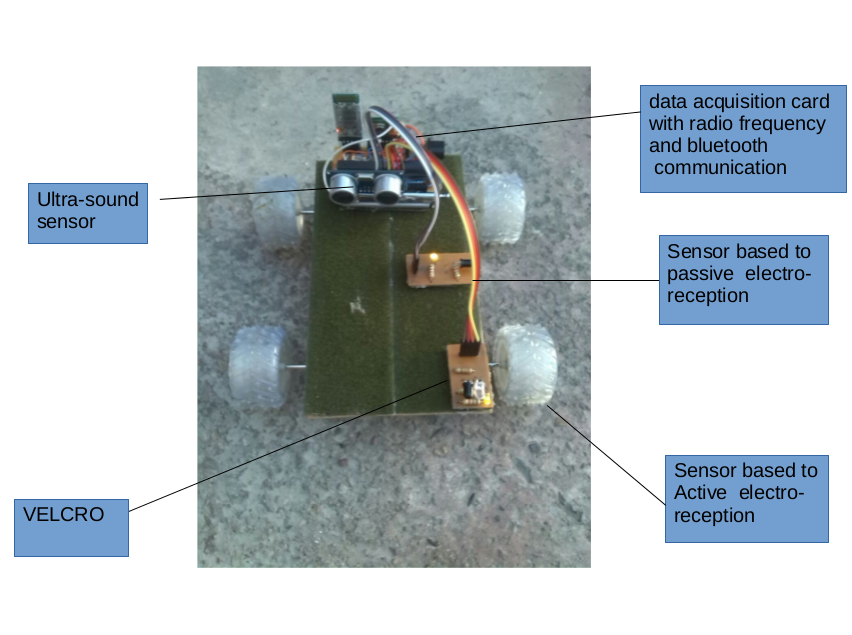
\includegraphics[width=7cm, height=5.0cm, angle=0]{carro.png}}
  \caption{\footnotesize Vehículo motorizado FREEinfraROSI. Autor (2017).}
  \label{fig:carro}  
\end{figure}

\section{Taller IoT}
En la ultima parte de la conferencia se aborda el tema de hardware libre con microcontroladores de la familia Atmega entre los cuales se destaca la placa \texttt{Arduino Uno} la cual se observa en la figura \ref{fig:Arduino}; y el módulo wifi \texttt{ESP 8266} el cual se muestra en la figura \ref{fig:ESP},se combinan estas dos tecnologías para el desarrollo de proyectos automatizados con internet
\\
\begin{figure}[htb]
  \centering
\setlength\fboxsep{0pt}
\setlength\fboxrule{0.5pt}
\fbox{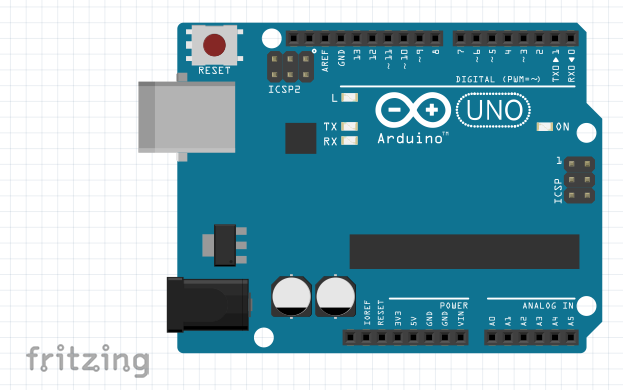
\includegraphics[width=7cm, height=5.0cm, angle=0]{arduino.png}}
  \caption{\footnotesize Placa micro controladora Arduino uno. Fritzing.}
  \label{fig:Arduino}  
\end{figure}

\begin{figure}[htb]
  \centering
\setlength\fboxsep{0pt}
\setlength\fboxrule{0.5pt}
\fbox{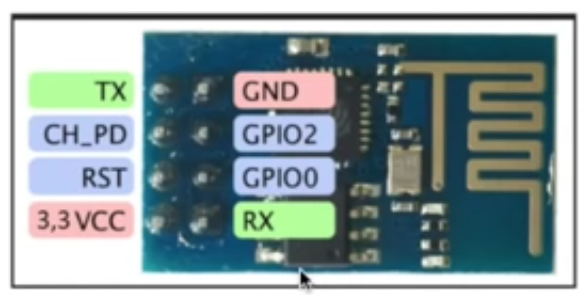
\includegraphics[width=7cm, height=5.0cm, angle=0]{ESP8266.png}}
  \caption{\footnotesize Imagen  del módulo \texttt{ESP8266}, tomada de la pagina oficial del proyecto  arduino  IDE.}
  \label{fig:ESP}  
\end{figure}

Básicamente se abordan los temas  de las conexiones del módulo \texttt{ESP8266}, sus conexiones con la placa arduino y controlado a través de comandos \texttt{AT} como se muestra en la figura \ref{fig:AT}; para todo esto el equipo de \texttt{Opensai} dispuso de un \texttt{web server} con conexión inalámbrica para los asistentes a este evento, lo cual hizo que la charla fuera muy dinámica e interactiva.
\\

\begin{figure}[htb]
  \centering
\setlength\fboxsep{0pt}
\setlength\fboxrule{0.5pt}
\fbox{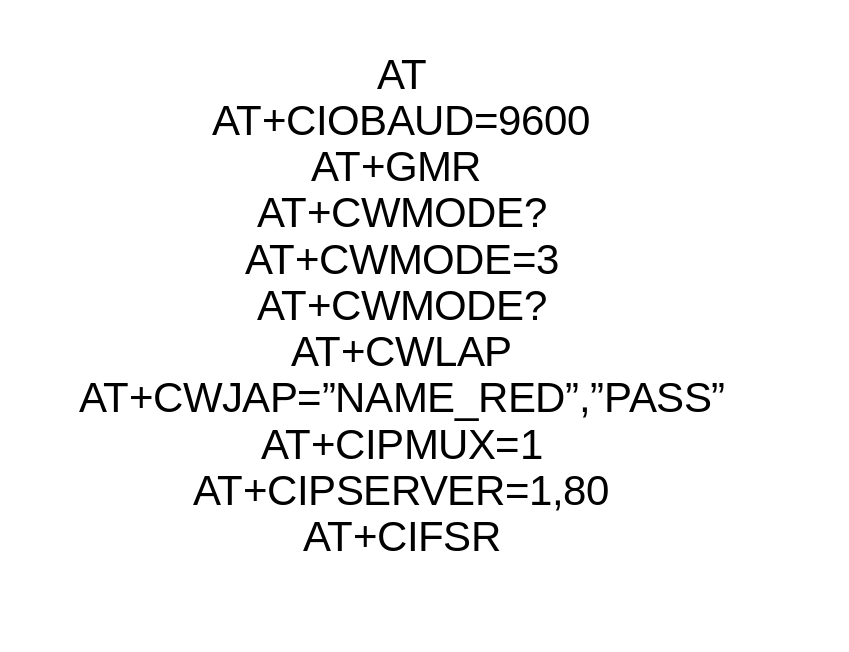
\includegraphics[width=7cm, height=5.0cm, angle=0]{AT-COMAND.png}}
  \caption{\footnotesize Comandos AT para control del dispositivo \texttt{ESP8266}; imagen tomada de la documentación del módulo.}
  \label{fig:AT}  
\end{figure}

El equipo de \texttt{Opensai}, agradece a la \texttt{Universidad Minuto de Dios}, por la invitación a este tipo de eventos y para terminar se muestran las gafas \texttt{smart glass BT-200 de EPSON} al auditorio y permite que el publico interactué con las mismas, como se muestra en la figura \ref{fig:gafas}.

\begin{figure}[htb]
  \centering
\setlength\fboxsep{0pt}
\setlength\fboxrule{0.5pt}
\fbox{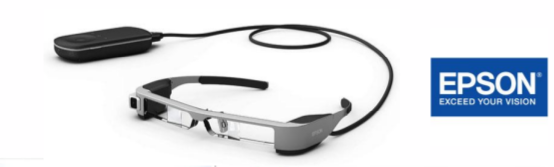
\includegraphics[width=7cm, height=5.0cm, angle=0]{epson.png}}
  \caption{\footnotesize \texttt{smart glass BT-200 de EPSON}, imagen tomada de la pagina oficial de EPSON. }
  \label{fig:gafas}  
\end{figure}




\bibliographystyle{apacite}
\bibliography{referencias}
\end{document}





